\section{Results}
\label{sec:results}

The goal of the chosen methodologies (see \hyperref[sec:methodology]{Section \ref*{sec:methodology}}) allows for answering of the \hyperref[rq:1]{(sub)research questions}. First, the results of the questionnaire survey is described (see \hyperref[sec:survey_analysis]{Section \ref*{sec:survey_analysis}}) and key insights into the air quality monitor data collection are presented (see \hyperref[sec:monitor_analysis] {Section \ref*{sec:monitor_analysis}}) to answer \hyperref[subq:1]{SQ\ref*{subq:1}}. Then, the developed prototype will be presented in section (see \hyperref[sec:prototype_results]{Section \ref*{sec:prototype_results}}), which addresses \hyperref[subq:2]{SQ\ref*{subq:2}} and the results from the evaluation sessions will be summarized in (see \hyperref[sec:evaluation_results]{Section \ref*{sec:evaluation_results}}) to address \hyperref[subq:3]{SQ\ref*{subq:3}}.

\subsection{Survey analysis}
\label{sec:survey_analysis}

The following section presents the outcomes of the survey conducted to assess various aspects related to occupants' activity, IAQ awareness, satisfaction, perception, and health impacts among Lab42 building occupants. The survey responses indicate that occupants have limited awareness of IAQ but generally perceive it as acceptable (see \hyperref[fig:likert-scales-survey]{Figure \ref*{fig:likert-scales-survey}}). This perception is attributed mainly to the building's spacious open areas and the presence of planters, which collectively contribute to satisfactory IAQ levels.

\begin{figure}[H]
    \centering
    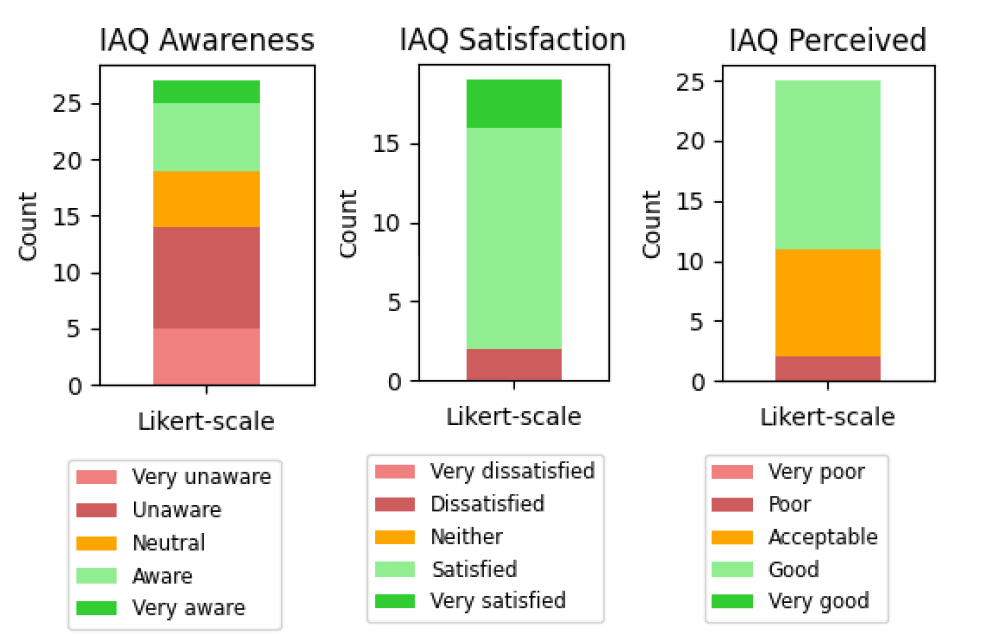
\includegraphics[width=0.5\textwidth]{IAQ_LIkert-Scales_Survey.jpg}
    \caption{Likert scales of IAQ awareness, perception and satisfaction of the questionnaire survey with occupant count}
    \label{fig:likert-scales-survey}
\end{figure}

\subsubsection{Activity and occupancy}

The first set of survey questions focused on activity and occupancy within the Lab42 building. On average, respondents used the Lab42 building three times per week for various activities ($min$=1, $max$=5, $mdn$=3). Usage varied, with some occupants frequenting the building only once per week while others used it all five working days per week. Most survey respondents were located on the ground floor ($f$=10) and the first floor ($f$=15), as opposed to the second floor. This is by design of the building where the ground and first floors are designated as the 'open area' and part of the atrium, which are designed for informal co-working and learning spaces. Most occupants described the overall occupancy as moderate ($f$=16), with fewer stating it was either crowded or not crowded at all.

\subsubsection{Awareness, perceived and satisfaction}

The second set of questions involved three Likert scales assessing perceived IAQ, awareness of IAQ, and satisfaction with IAQ. Over half of the occupants reported low awareness of IAQ in their current space, identifying as very unaware ($f$=5), unaware ($f$=9), or neutral ($f$=5). Only a minority of occupants were aware or very aware of IAQ. Despite this low awareness, most occupants perceived the IAQ as acceptable ($f$=9) or good ($f$=14), with nearly all expressing satisfaction, either satisfied ($f$=8) or very satisfied ($f$=14).


\subsubsection{Health and cognitive symptons}

The third set of questions aimed to identify if users experienced health or cognitive symptoms related to IAQ. The majority of participants reported no health ($f$=21) or cognitive ($f$=15) symptoms. A small percentage experienced health issues such as headaches and nausea, while a larger percentage reported cognitive symptoms like difficulty focusing or fatigue. These results are inconclusive, as linking these symptoms to IAQ directly is challenging.

\subsubsection{Open-ended air quality description}
The open-ended responses revealed that many occupants perceived the IAQ positively, often attributing this to the openness of the atrium space. For instance:

\begin{quote}
P11: "[...] think it is good, [...] although I must say that this is mostly based on the large amount of open space in the building"
\end{quote}

\begin{quote}
P8: " [...] feel like in this building the air quality is really good, mainly because of the impression the high ceilings give"
\end{quote}

\begin{quote}
P13: "I like the air quality. This may also be because I sit close to the door, and the ceiling is high."
\end{quote}

Additionally, many occupants mentioned the presence of hanging planters and greenery as factors contributing to their perception of sufficient IAQ:

\begin{quote}
P16: "[..] I also see green plants around me, of which I think they are real."
\end{quote}

\begin{quote}
P14: "[...] and the hanging plants that are present.
\end{quote}

These qualitative insights underscore the importance of spatial design and greenery in influencing occupants' perceptions of IAQ.

\subsection{Air Quality Monitors}
\label{sec:monitor_analysis}

The collected data logs were exported from the monitoring devices and analyzed with a primary focus on CO2 concentrations, as this parameter significantly impacts indoor air quality (IAQ). CO2 levels accumulate due to human respiration, and air quality is heavily influenced by room occupancy. The analysis of these logs reveals occupancy patterns typical of scheduled meetings and the development of suboptimal CO2 concentrations within the meeting rooms frequently exceeding the optimal threshold of 600 \textit{ppm} (see \hyperref[appendix:monitor-data]{Appendix \ref*{appendix:monitor-data}}).

\begin{figure}[h]
    \centering
    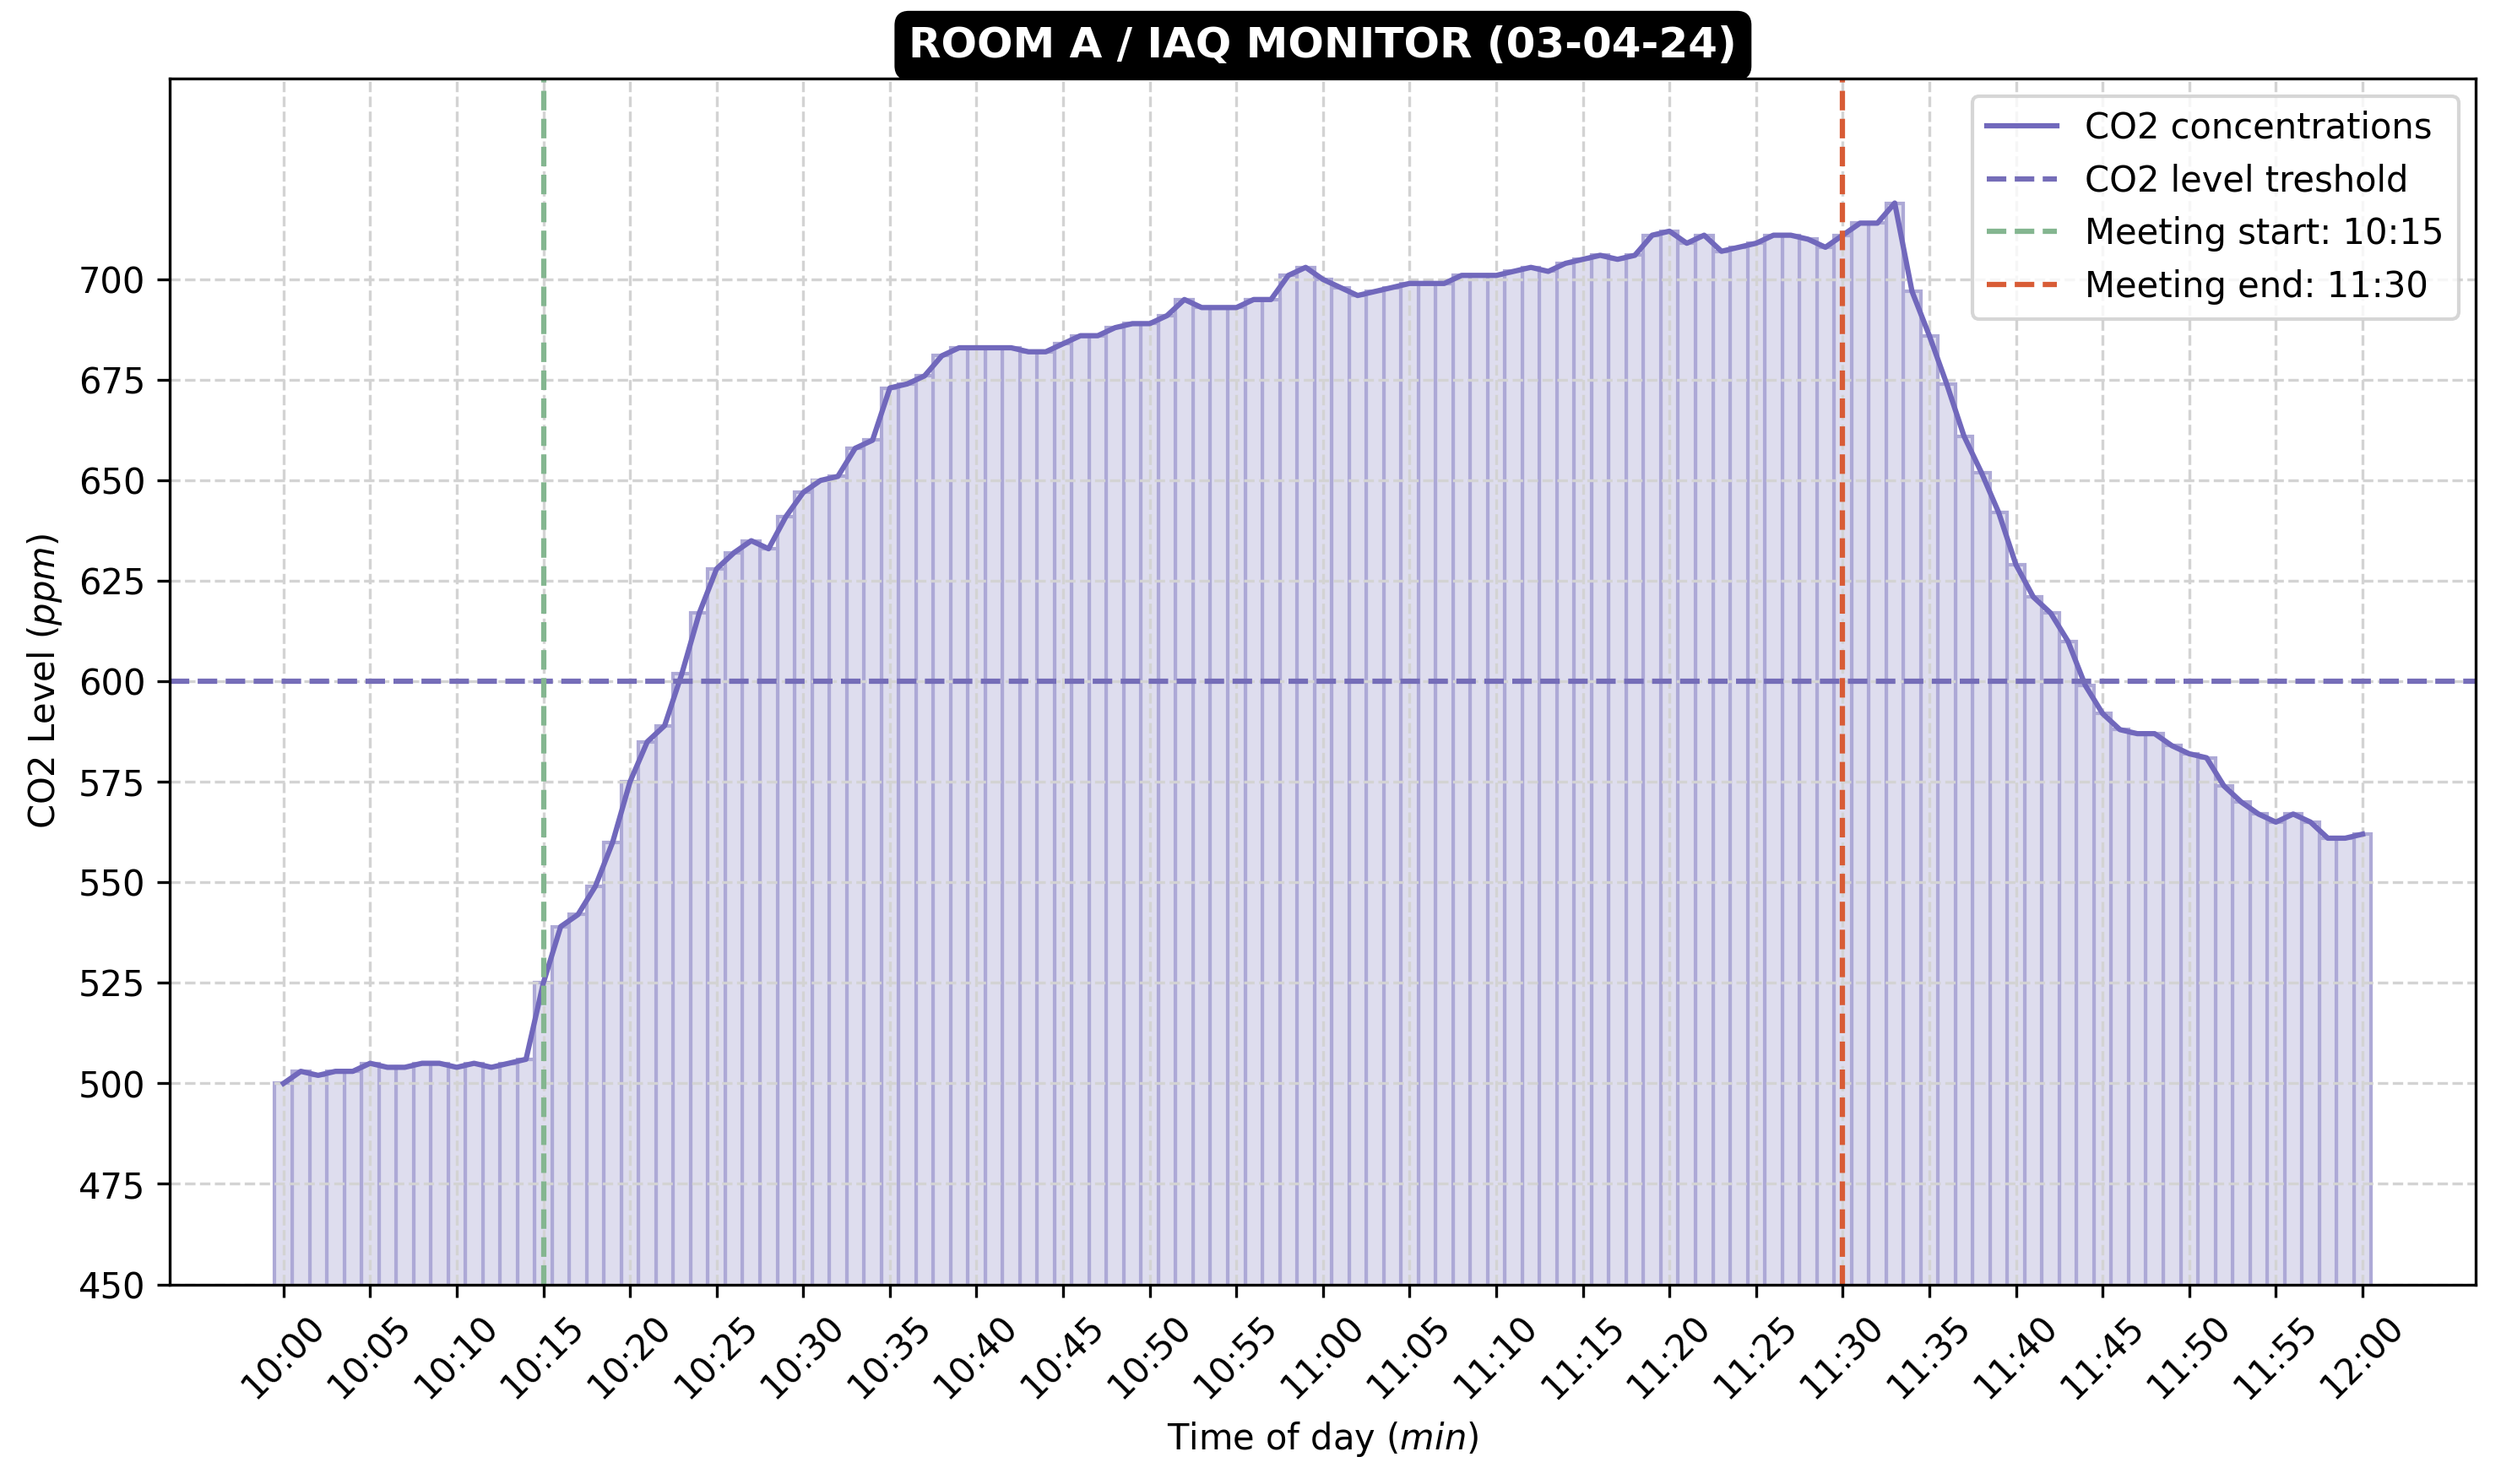
\includegraphics[width=0.5\textwidth]{room-a-monitor-meeting-spike-single.png}
    \caption{Line chart of a single meeting in the small Room A showing the start and end time of the meeting}
    \label{fig:room-a-spike}
\end{figure}

\subsubsection{Single meeting CO2 development}

A sample of CO2 concentrations (see \hyperref[fig:room-a-spike]{Figure \ref*{fig:room-a-spike}}) in a single meeting shows CO2 levels over time, with the x-axis indicating time in minutes and the y-axis showing CO2 concentrations in ppm. The ideal maximum threshold of 600 \textit{ppm} is marked on the x-axis. Two colored lines on the y-axis denote the start and end times of the meeting. The data indicates that within fifteen minutes of the meeting starting, CO2 levels reach suboptimal levels and continue to rise, stabilizing around 950 \textit{ppm}, which is the peak concentration for the meeting. Continuous exposure to CO2 levels between 800 \textit{ppm} and 1000 \textit{ppm}, or higher is considered detrimental to cognitive functions. After the meeting
concluded, CO2 concentrations gradually decreased to the baseline
level of 450 \textit{ppm} as occupants left the room.

\begin{figure}[h]
    \centering
    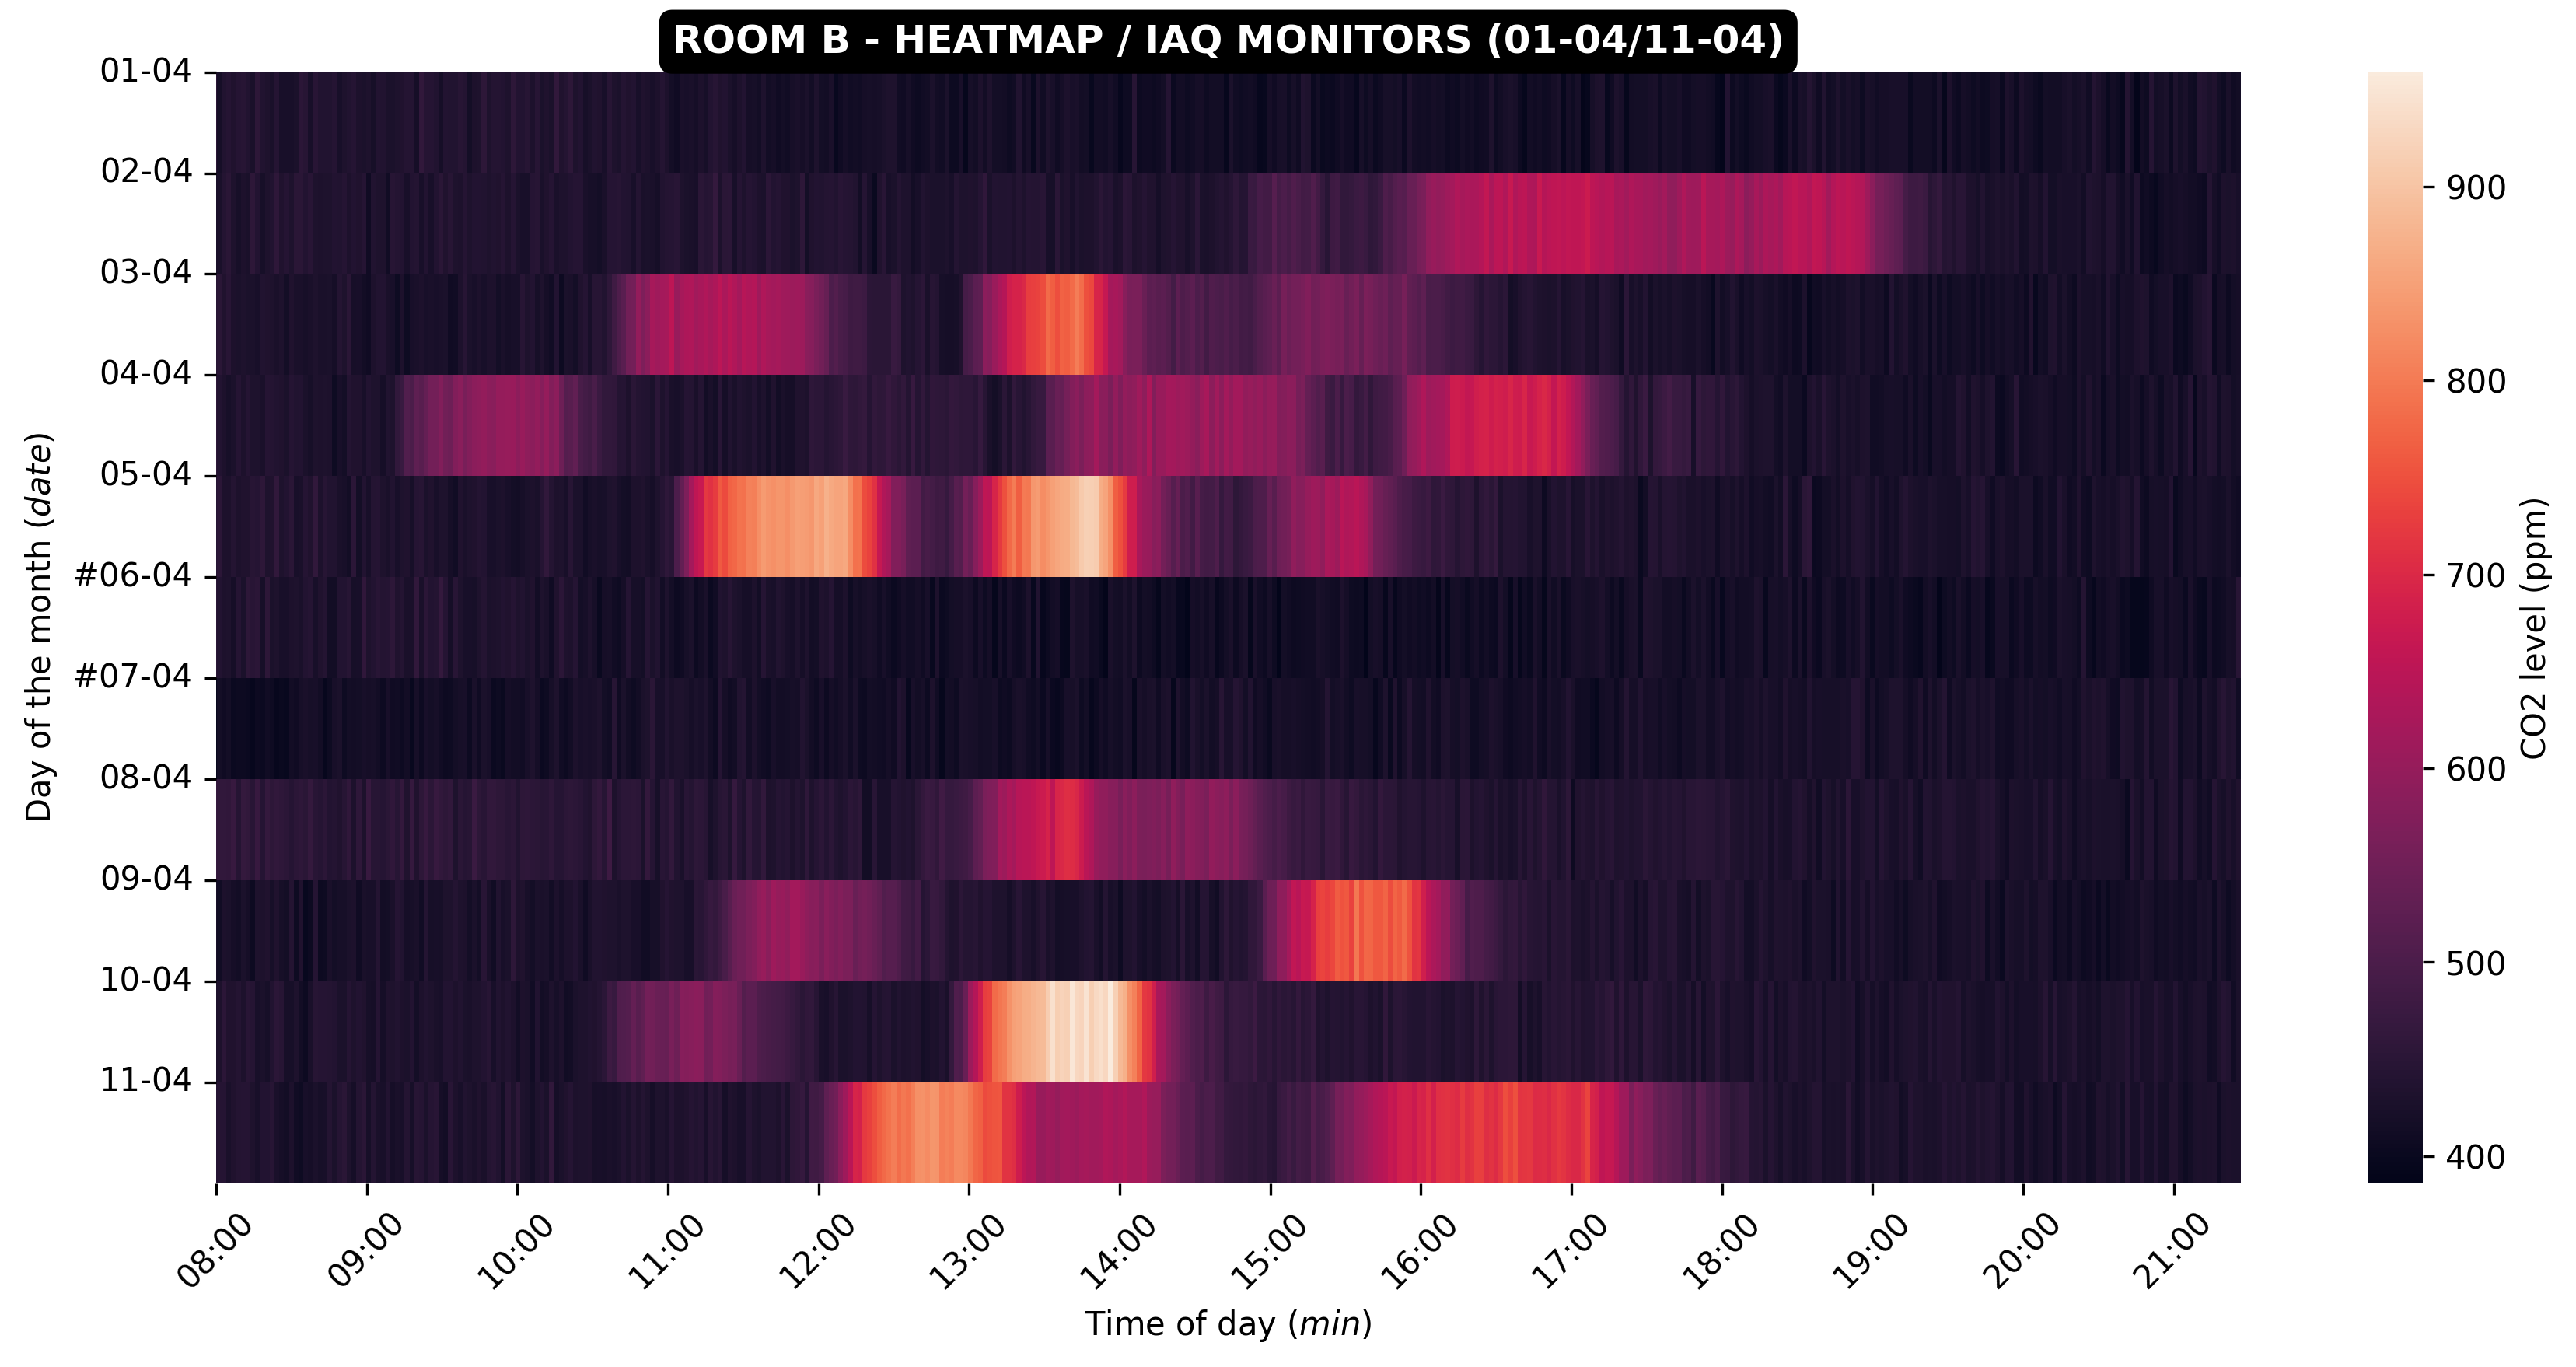
\includegraphics[width=0.5\textwidth]{room-b-monitor-heatmap.png}
    \caption{Heatmap of ten days of data logs from Room B showing the peaks of CO2 concentrations monitored }
    \label{fig:room-b-heatmap-chart}
\end{figure}

\subsubsection{Regular day CO2 development}

The visualization in \hyperref[appendix:monitor-data]{Appendix \ref*{appendix:monitor-data}} depicts CO2 concentration spikes throughout a typical day with multiple meetings. The x-axis plots CO2 levels, while the y-axis represents the full day within the building’s opening hours. Data from randomly sampled days show that most meetings occur between late morning (11:00) and late afternoon (17:00), roughly two hours after the building opens and four hours before it closes. There are outliers, with some meetings occurring early in the morning right after opening and occasionally extending into the evening.

\subsubsection{Meeting schedule CO2 development}

A heatmap of ten days of CO2 concentration monitoring (see \hyperref[fig:room-b-heatmap-chart]{Figure \ref*{fig:room-b-heatmap-chart}}) reveals that typically two or three meetings occur each day, usually lasting around one hour. Most of these meetings result in CO2 levels exceeding the 600 ppm threshold. Line plots and heatmaps suggest that Room B, being larger, is more frequently used and reaches higher CO2 concentrations. However, these results lack conclusiveness because they depend on the specific context and periods during which data was collected and monitors were installed.


\subsection{Prototype}
\label{sec:prototype_results}

Based on the requirements, data physicalization design principles, and exploration of concept models, a high-fidelity (hi-fi) prototype was developed. This prototype serves as a proof-of-concept for the physical design solution and was used in the user study for evaluation.

\subsubsection{Concept description}

The prototype, named \textit{Bluebird}, is a hanging kinetic sculpture inspired by natural materials and the shapes of hanging planters. It encodes indoor air quality (IAQ) data to foster a relationship with nature. Designed to be hung from the ceiling in small to medium-sized rooms, it changes based on real-time air quality data, engaging occupants with the air quality levels. The artefict features strings (representing plant branches) that elongate or contract, simulating plant growth, and leaves that move to indicate air freshness and movement. The design philosophy employs calm technology to minimize interruption costs \cite{case_calm_2016}. Unlike existing solutions, Bluebird provides predictions and historical data, not just feedback on current conditions when CO2 levels are high.

\subsubsection{Experimental set-up}

The prototype was installed \textit{in situ} in one of the meeting rooms in the building (see \hyperref[fig:photograph-prototype]{Figure \ref*{fig:photograph-prototype}}). Four dimensions were derived from the literature to describe the prototype: \textit{properties, environment, interaction, and representation} \cite{sauve_physecology_2022, hornecker_design_2023, anhalt_university_germany_design_2022}.

\begin{itemize}
  \item \textbf{Properties}: The technology-assisted physicalization uses explicit visual variables such as size, position, timing, and movement where occupants visually see the strings becoming larger (height) and leaves moving to change the visual arrangement (movement), all based on the temporal frequency of CO2 concentrations.
  \item \textbf{Environment}: The design uses associative metaphors through shapes and movement, resembling organic forms found in nature (shape and form). It is a medium to large-scale (50 - 150 cm) physicalization, placed semi-publicly within the open building context.
  \item \textbf{Interaction}: The artifact communicates environmental data, aiding in understanding and encouraging reflection. It features indirect interaction, changing based on occupant activity.
  \item \textbf{Representation}: The dataset is dynamic, streaming real-time environmental data from building sensors and outputting categorical data on CO2 concentration variations.
\end{itemize}

\subsubsection{Electronics and components}

The prototype is controlled by an Arduino Uno R3 \footnote{https://store.arduino.cc/products/arduino-uno-rev3} microcontroller with a PWM 6-Channel Servo Driver \footnote{https://learn.adafruit.com/16-channel-pwm-servo-driver?view=all} operating six 360° MG90S type Micro Servo Motors \footnote{https://www.towerpro.com.tw/product/mg90s-3/}. These motors, attached to pulleys with paracord ropes, simulate plant growth by moving the strings up and down. All electronics are integrated into the back of a wooden board, making the device stand-alone, movable, and modular for installation in other spaces.

\subsubsection{Crafting technologies and materials}
The strings, leaves, and housings for the electronics and mechanical hardware were created using additive manufacturing (3D printing) with Fused Deposition Modeling (FDM) techniques a fabrication technique commonly found in data physicalizations \cite{anhalt_university_germany_design_2022}. Polylactic acid (PLA) plastic filament in various colors was used. The electronics enclosures and plant models were designed using computer-aided design (CAD) software. To create leaf-like representations, custom properties were defined in the 3D printing software (slicing) to remove top and bottom layers, resulting in a thin infill layer.

\subsubsection{System Architecture and software}

The microcontroller runs custom firmware written in Arduino code\footnote{\url{https://www.arduino.cc/reference/en/}} (similar to C++), receiving real-time data from air quality monitors using the Lab42 internal building API (see \hyperref[appendix:api-sample-data]{Appendix \ref*{appendix:api-sample-data}}). Via an ESP32 (NodeMCU)\footnote{\url{https://www.nodemcu.com/}}, the data is sent over UART to the Arduino controller. This arrangement of hardware is commonly found in Internet of Things (IoT) architecture set-ups and follows the notion of Edge Computing with a (1) sensing, (2) networking, (3) processing, and (4) application layer \cite{li_edge-oriented_2019, idrees_edge_2018}. Custom library functions were written to calculate string movements. The current (\( C_{\text{current}} \) ) and \( C_{\text{previous}} \) CO2 concentrations are stored, with the difference calculated and mapped to a movement time \( t_{\text{movement}} \) in milliseconds. Based on whether the integer is negative or positive and a multiplication factor, the servo motors spin either clockwise (growing) or counterclockwise (shrinking) the ropes.


\subsection{Evaluation}
\label{sec:evaluation_results}

The prototype-led evaluation sessions (see \hyperref[sec:questionnaire]{Section \ref*{sec:questionnaire}}) were held to assess the understanding of the data physicalization with a focus on how occupants perceive the data embedded in the physical representation, usability test the prototype for design improvements and suggestions and gain insight into its effectiveness.

\begin{figure}[b]
    \centering
    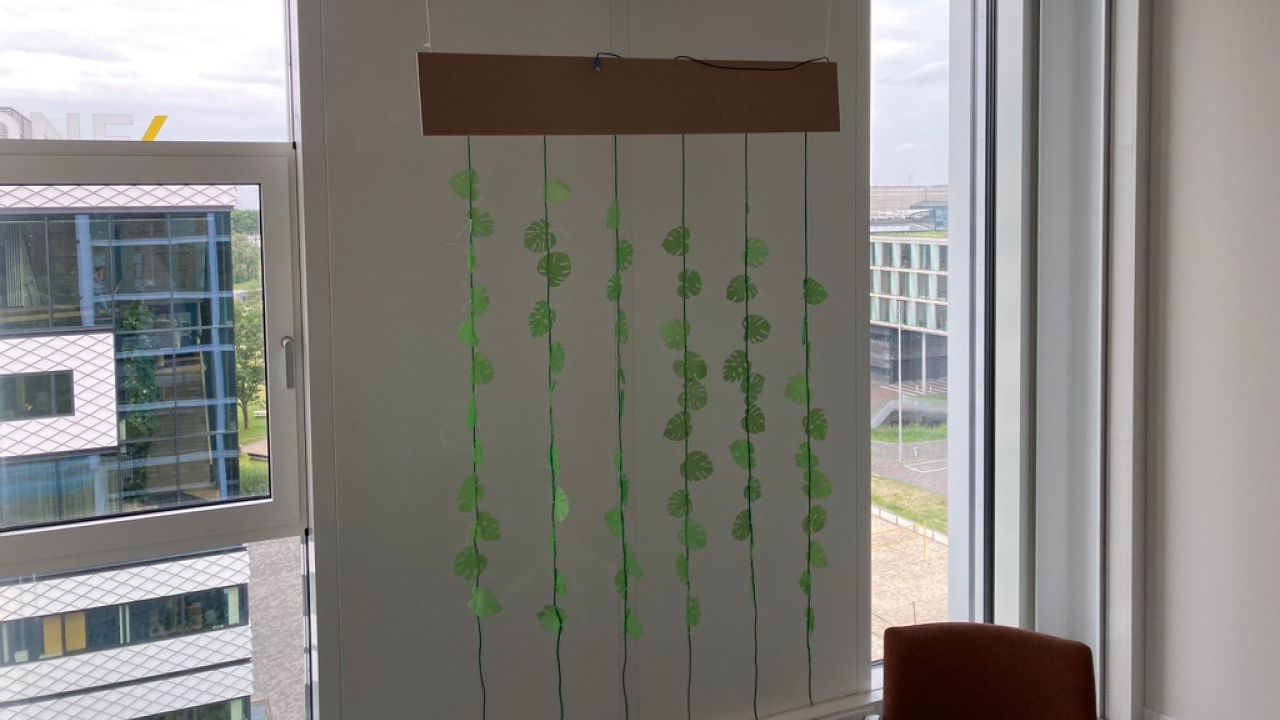
\includegraphics[width=0.45\textwidth]{prototype_installed.jpg}
    \caption{Photograph of the prototype installed in the room during an evaluation session with a participant }
    \label{fig:photograph-prototype}
\end{figure}

\subsubsection{Usefulness and aesthetic impressions (engagement)}

All participants (see \hyperref[appendix:participants]{Appendix \ref*{appendix:participants}}) indicated during the usability test or through their scores that they enjoyed viewing the data physicalization and gained valuable insights about indoor air quality from its display in the meeting room. They also reported a high likelihood of taking preventive action based on these insights. Opinions on the materials and aesthetics were mixed: \textit{P2} suggested adding more strings for granular data, while others found the current number sufficient. \textit{P3} proposed more variation in the leaves' shapes and densities for aesthetics, but this was not a shared view. \textit{P2} and \textit{P3} also recommended that the wooden board and materials be better
integrated into the room’s interior by hiding it in the ceiling
or covering it to match the color scheme.

\begin{quote}
P3: "I also think the leaves are too artificial, I would prefer more organic materials. [..] The wooden board feels off [...]"
\end{quote}

\subsubsection{Perceived data and learnability (understanding)}
Almost all participants, except for \textit{P2}, indicated that the prototype's learnability on initial view is high. They noted that without clear instructions, the physicalization is too abstract in conveying information about indoor air quality, as reflected in generally low scores for statement S2 (see \hyperref[appendix:implications]{Appendix \ref*{appendix:implications}}) from the survey. Design recommendations mostly evolved around helping occupants better understand the physicalization with better onboarding for example, in the form of a scannable QR code or text instructions on the wooden board.

\begin{quote}
P1: "[...] on initial view it's a bit of a puzzle what IAQ properties it communicates. But once you understand it and learn it I assume it will have a long-term behavior change effect."
\end{quote}


\subsubsection{Design Improvements and recommendations (effectiveness)}

Participants suggested numerous design improvements and recommendations during usability testing. These suggestions, coded and categorized, primarily aimed to increase the physicalization's overall effectiveness (see \hyperref[appendix:improvements]{Appendix \ref*{appendix:improvements}}). \textit{P1, P2, P3 } emphasized that the positioning of the physicalization within the room significantly impacts its effectiveness for all occupants. Additionally, \textit{P1, P3} recommended color-coding or labeling the leaves indicating the history, current, and future predictions of CO2 concentrations to make this property more apparent.

\begin{quote}
P3: "I feel like the positioning within the room is important. [...] You want the physicalization visible to all occupants within the room. Putting it next to the door or one wall makes people sit with their back to it."
\end{quote}